%%%%%%%%%%%%%%%%%%%%%%%%%%%%%%%%%%%%%%%%%%%%%%%%%%%%%%%%%%%%
% File: hw.tex 						   %
% Description: LaTeX template for homework.                %
%
% Feel free to modify it (mainly the 'preamble' file).     %
% Contact hfwei@nju.edu.cn (Hengfeng Wei) for suggestions. %
%%%%%%%%%%%%%%%%%%%%%%%%%%%%%%%%%%%%%%%%%%%%%%%%%%%%%%%%%%%%

%%%%%%%%%%%%%%%%%%%%%%%%%%%%%%%%%%%%%%%%%%%%%%%%%%%%%%%%%%%%%%%%%%%%%%
% IMPORTANT NOTE: Compile this file using 'XeLaTeX' (not 'PDFLaTeX') %
%
% If you are using TeXLive 2016 on windows,                          %
% you may need to check the following post:                          %
% https://tex.stackexchange.com/q/325278/23098                       %
%%%%%%%%%%%%%%%%%%%%%%%%%%%%%%%%%%%%%%%%%%%%%%%%%%%%%%%%%%%%%%%%%%%%%%

\documentclass[11pt, a4paper, UTF8]{ctexart}
%%%%%%%%%%%%%%%%%%%%%%%%%%%%%%%%%%%
% File: preamble.tex
%%%%%%%%%%%%%%%%%%%%%%%%%%%%%%%%%%%

\usepackage[top = 1.5cm]{geometry}

% Set fonts commands
\newcommand{\song}{\CJKfamily{song}} 
\newcommand{\hei}{\CJKfamily{hei}} 
\newcommand{\kai}{\CJKfamily{kai}} 
\newcommand{\fs}{\CJKfamily{fs}}

\newcommand{\me}[2]{\author{{\bfseries 姓名:}\underline{#1}\hspace{2em}{\bfseries 学号:}\underline{#2}}}

% Always keep this.
\newcommand{\noplagiarism}{
  \begin{center}
    \fbox{\begin{tabular}{@{}c@{}}
      请独立完成作业,不得抄袭。\\
      若参考了其它资料,请给出引用。\\
      鼓励讨论,但需独立书写解题过程。
    \end{tabular}}
  \end{center}
}

% Each hw consists of three parts:
% (1) this homework
\newcommand{\beginthishw}{\part{作业}}
% (2) corrections (Optional)
\newcommand{\begincorrection}{\part{订正}}
% (3) any feedback (Optional)
\newcommand{\beginfb}{\part{反馈}}

% For math
\usepackage{amsmath}
\usepackage{amsfonts}
\usepackage{amssymb}

% Define theorem-like environments
\usepackage[amsmath, thmmarks]{ntheorem}

\theoremstyle{break}
\theorembodyfont{\song}
\theoremseparator{}
\newtheorem*{problem}{题目}

\theorempreskip{2.0\topsep}
\theoremheaderfont{\kai\bfseries}
\theoremseparator{:}
% \newtheorem*{remark}{注}
\theorempostwork{\bigskip\hrule}
\newtheorem*{solution}{解答}
\theorempostwork{\bigskip\hrule}
\newtheorem*{revision}{订正}

\theoremstyle{plain}
\newtheorem*{cause}{错因分析}
\newtheorem*{remark}{注}

\theoremstyle{break}
\theorempostwork{\bigskip\hrule}
\theoremsymbol{\ensuremath{\Box}}
\newtheorem*{proof}{证明}

\renewcommand\figurename{图}
\renewcommand\tablename{表}

% For figures
% for fig with caption: #1: width/size; #2: fig file; #3: fig caption
\newcommand{\fig}[3]{
  \begin{figure}[htp]
    \centering
      \includegraphics[#1]{#2}
      \caption{#3}
  \end{figure}
}

% for fig without caption: #1: width/size; #2: fig file
\newcommand{\fignocaption}[2]{
  \begin{figure}[htp]
    \centering
    \includegraphics[#1]{#2}
  \end{figure}
}  % modify this file if necessary

%%%%%%%%%%%%%%%%%%%%
\title{第十二讲:偏序关系和格}
\me{丁保荣}{171860509}
\date{\today}     % you can specify a date like ``2017年9月30日''.
%%%%%%%%%%%%%%%%%%%%
\begin{document}
\maketitle
%%%%%%%%%%%%%%%%%%%%
\noplagiarism	% always keep this
%%%%%%%%%%%%%%%%%%%%
\beginthishw	% begin ``this homework (hw)'' part

%%%%%%%%%%
\begin{problem}[SM: 14.32]
Let \(B = \{a, b, c, d, e, f \}\) be ordered as in Fig.14-17(b).

(a) Find all minimal and maximal elements of B.

(b) Does B have a first or last element?

(c) List two and find the number of consistent enumerations of B into the set \(\{1, 2, 3, 4, 5, 6\}\).
\end{problem}
\begin{solution}
(a) mimimal elements: d and f\\
maximal elements: a\\
(b) It doesn;t have a first element, but it has a last element.\\
(c) \\
f: f(a)=6, f(b)=5, f(c)=4, f(d)=3, f(e)=2, f(f)=1\\
f: f(a)=6, f(b)=4, f(c)=5, f(d)=3, f(e)=2, f(f)=1\\
The number of consistent enumerations of B is 11.
\end{solution}


\begin{problem}[SM: 14.44]
Suppose the following are three consistent enumerations of an ordered set \(A = \{a, b, c, d\}\):
\[[(a, 1), (b, 2), (c, 3), (d, 4)], [(a, 1), (b, 3), (c, 2), (d, 4)], [(a, 1), (b, 4), (c, 2), (d, 3)]\]
Assuming the Hasse diagram D of A is connected, draw D.
\end{problem}
\begin{solution}
\fig{width = 0.70\textwidth}{14.44.JPG}{Hasse diagram}
\end{solution}



\begin{problem}[SM: 14.46]
Consider the English alphabet \(A = \{a, b, c, . . . , y, z\}\) with the usual (alphabetical) order. Recall A∗ consists of all words in A. Let L consist of the following list of elements in A∗:
\[\mbox{gone, or, arm, go, an, about, gate, one, at, occur}\]

(a) Sort L according to the short-lex order, i.e., first by length and then alphabetically.

(b) Sort L alphabetically.
\end{problem}
\begin{solution}
(a) an, at, go, or, arm, one, about, gate, gone, occur.\\
(b) about, an, arm, at, gate, go, gone, occur, one, or.\\
\end{solution}



\begin{problem}[SM: 14.58]
Show that the isomorphism relation \(A \cong B\) for ordered sets in an equivalence relation, that is:

(a) \(A \cong A\) for any ordered set A. (b) If \(A \cong B\), then \(B \cong A\). (c) If \(A \cong B\) and \(B \cong C\), then \(A \cong C\).
\end{problem}
\begin{solution}
(a) we can define f: A$\rightarrow$A by f(a)=a, and we can easily note that this remains the order relations.\\
(b) For A$\cong$B, we can find a bijective function f: A$\rightarrow$B that satisfies (i) if a>b, then f(a)>f(b) (ii) if a||b then f(a)||b. Therefore there is a bijective function f$^{-1}$, which also satisfies (i) if u>v(f(a)>f(b)), then f$^{-1}$(u)>f$^{-1}$(v) (a>b) and (ii) if u||v(f(a)||f(b)), then f$^{-1}$(u)||f$^{-1}$(v) (a||b)\\
(c) for A$\cong$B and B$\cong$C, we can find f: A$\rightarrow$B and g: B$\rightarrow$C that satisfy the two properties.\\
Therefore we can define F: A$\rightarrow$C by F=g$\circ$f\\
if a>b, then f(a)>f(b), then g(f(a))>g(f(b)), namely F(a)>F(b)\\
If a||b, then f(a)||f(b), then g(f(a))||g(f(b)), namely F(a)||F(b)\\
Therefore F also satisfies the two properties.\\
Therefore A$\cong$C
\end{solution}



\begin{problem}[SM: 14.62]
Suppose A and B are well-ordered isomorphic sets. Show that there is only one similarity mapping \(f: A → B\).
\end{problem}
\begin{solution}
Since A and B are well-ordered isomorphic sets, the elements in A(or B) are all comparable and we can find a bijective function f: A$\rightarrow$B\\
A and B are linearly ordered. Therefore we can form A into a chain and B into a chain.\\
and the mapping from A to B should be parallel (as f has to perserve the order relation).\\
If there is another similarity mapping g, g must be have lines crossed, and it breaks the order relation, therefore g is not a similarity mapping.\\
Therefore there is only one similarity mapping \(f: A → B\).\\
\end{solution}




\begin{problem}[SM: 14.66]
\par
\begin{center}
    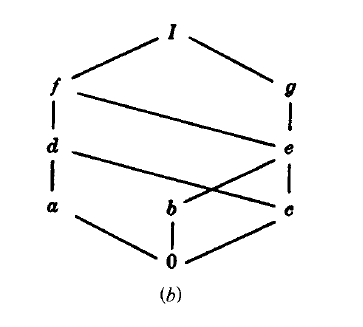
\includegraphics[width=6cm]{tupian1.png}
\end{center}
Consider the lattice M in Fig.14-19(b).

(a) Find all join-irreducible elements.

(b) Find the atoms.

(c) Find complements of a and b, if they exist.

(d) Express each x in M as the join of irredundant join-irreducible elements.

(e) Is M distributive? Complemented?
\end{problem}
\begin{solution}
(a) a,b,c,g,0\\
(b) a,b,c\\
(c) a:g   b:none;\\
(d) I=a$\vee$g, f=a$vee$b, d=a$vee$c, a=a$\vee$0, e=b$\vee$c, g=b$\vee$g, c=c$\vee$0, b=b$\vee$0, 0=0$\vee$0\\
(e)it is not distributive or complemented.
\end{solution}



\begin{problem}[SM: 14.70]
Consider the lattice \(D_{60} = \{1, 2, 3, 4, 5, 6, 10, 12, 15, 20, 30, 60\}\), the divisors of 60 ordered by divisibility.

(a) Draw the diagram of \(D_{60}\).

(b) Which elements are join-irreducible and which are atoms?

(c) Find complements of 2 and 10, if they exist.

(d) Express each number x as the join of a minimum number of irredundant join irreducible elements.
\end{problem}
\begin{solution}
(a) \fig{width = 0.70\textwidth}{14.70.JPG}{diagram}\\
(b) join-irreducible: 1,2,3,4,5\\
atoms: 2,3,5\\
(c) complement of 2 doesn't exist.\\
complement of 10 doesn't exist.\\
(d) 60=5$\vee$4$\vee$3, 30=2$\vee$3$\vee$5, 20=4$\vee$5, 15=3$\vee$5, 12=3$\vee$4, 10=2$\vee$5, 6=2$\vee$3.

\end{solution}



\begin{problem}[SM: 14.75]
A lattice M is said to be modular if whenever \(a \leq c\) we have the law
\[a \vee (b \wedge c) = (a \vee b) \wedge c\]

(a) Prove that every distributive lattice is modular.

(b) Verify that the non-distributive lattice in Fig.14-7(b) is modular; hence the converse of (a) is not true.

(c) Show that the nondistributive lattice in Fig.14-7(a) is non-modular.(In fact, one can prove that every non-modular lattice contains a sublattice isomorphic to Fig.14-7(a).)
\end{problem}
\begin{solution}
(a) because a$\le$c, then a$\vee$c=c\\
a$\vee$(b$\vee$c)=(a$\vee$b)$\wedge$(a$\vee$c)=(a$\vee$b)$\wedge$c.\\
Therefore every distributive lattice is modular.\\
(b) I$\ge$a, a$\vee$(b$\wedge$I)=I=(a$\vee$b)$\wedge$I. For b and c, it is similiar.\\
(c) c$\ge$a, a$\vee$(b$\wedge$c)=a while (a$\vee$b)$\wedge$c=c, therefore a$\vee$(b$\wedge$c)$\not=$(a$\vee$b)$\wedge$c. Therefore the non-distributive lattice in Fig.14-7(b) is modular, hence the converse of (a) is not true.

\end{solution}








%%%%%%%%%%
%%%%%%%%%%%%%%%%%%%%
\begincorrection	% begin the ``correction'' part (Optional)

%%%%%%%%%%
\begin{problem}[UD:13.5]
  Let x be a nonempty set and let A be a subset of X. We define the Characteristic function of the set A by
\begin{align}
X_{A}(x) = 
\begin{cases}
1 \qquad if \quad x \in A\\
0 \qquad if \quad x \in X \backslash A
\end{cases}
\end{align}

(a)Since this is called the characteristic function, it probably is a function, but check this carefully anyway.

(b)Determine the domain and range of this function. Make sure you look at all possibilities for A and X.
\end{problem}

\begin{cause}
  简述错误原因(可选)。
\end{cause}

% Or use the ``solution'' environment
\begin{revision}
(a)\\
(i) Since A is a subset of X, for every x$\in$X, there are two cases: x$\in$A or x$\in$X$\backslash$A\\
The two cases are defined in the $X_A$\\
(ii) Since A is a subset of X, for every x$\in$X, there are two cases: x$\in$A or x$\in$X$\backslash$A\\
(1) x$\in$A , the y is unique, namely 1\\
(2) x$\in$X$\backslash$A, the y is also unique, namely 0\\
$\therefore$ for every x$\in$X, the y it relates to is unique.\\
$\therefore$ $X_A$ satisfies (i) and (ii)\\
$\therefore$ $X_A$ is a well-defined function. \\
(b)\\
the domain of this function is X\\
(i) A=$\emptyset$, ran(f)=\{0\}\\
(ii) A=X, ran(f)=\{1\}\\
(iii) A $\not=$X and A$\not=\emptyset$, ran(f)=\{0,1\}\\

\end{revision}

\begin{problem}[UD:14.12]
Let a, b, c, and d be real numbers with \(a < b\) and \(c < d\). Define a bijection from the closed interval \([a,b]\) onto the closed interval \([c,d]\) and prove that your function is a bijection.
\end{problem}
\begin{revision}
f(x)=$\frac{d-c}{b-a}$(x-a) +c\\
Prove:\\
(1)if x1,x2$\in$[a,b] and f(x$_1$)=f(x$_2$), then $\frac{d-c}{b-a}$(x$_1$-a) +c=$\frac{d-c}{b-a}$(x$_2$-a) +c\\
$\therefore$ $\frac{d-c}{b-a}$(x$_1$-a)=$\frac{d-c}{b-a}$(x$_2$-a) \\
$\because$ a<b and c<d\\
$\therefore$ a-b<0, c-d<0\\
$\therefore$ x$_1$-a=x$_2$-a\\
$\therefore$ x$_1$=x$_2$\\
$\therefore$ this function is one-to-one\\
(2)for every y$\in$ [c,d], let f(x)=y\\
$\therefore$ $\frac{d-c}{b-a}$(x-a) +c=y\\
$\therefore$ x= $\frac{b-a}{d-c}$(y-c) +a\\
$\because$ y$\in$[c,d]\\
$\therefore$ x$\in$[a,b]\\
$\therefore$ for every y$\in$[c,d], we can find x$\in$[a,b] that satisfies y=f(x)\\
$\therefore$ this function is onto\\
Based on (1) and (2), this function is bijective.\\
\end{revision}
%%%%%%%%%%


\begin{problem}[UD:15.14]
Let A, B, C, and D be nonempty sets. Let \(f:A \rightarrow B\) and \(g:C \rightarrow D\) be functions.

(a) Prove that if f and g are one-to-one, then \(H: A \times C \rightarrow B \times D\) defined by 
\[H(a,b) = (f(a),g(c))\]
is a one-to-one function. (Check that it is one-to-one and a function.)
\end{problem}
\begin{remark}
一开始的部分先说明H是一个well-defined的function
\end{remark}
\begin{revision}
(a) \\
$\because$ f and g are one-to-one functions, \\
$\therefore$ for every a$\in$A and c$\in$C, we have there exist a u$\in$B that satisfies u=f(a) and a w$\in$B that satisfies w=g(c).\\
and if f(a)=f(b), then a=b, for g is the similarly\\
$\therefore$ H is a one-to=one function\\
\end{revision}


\begin{problem}[UD:16.21]
Suppose that \(f: X \rightarrow Y\) is a function, and let \(B_{1}\) and \(B_{2}\) be subsets of Y.

(b) Let f be a bijective function. Show that if \(f^{-1}(B_{1}) = f^{-1}(B_{2})\), then \(B_{1} = B_{2}\). Indicate clearly where you use one-to-one or onto. Did you use both?
\end{problem}
\begin{revision}
(b)\\ 
$\because$$f^{-1}(B_1)=f^{-1}(B_2)$\\
Let a$\in$ $f^{-1}(B_1)$,b$\in$$f^{-1}(B_2)$,x=f(a)$\in B_1$, y=f(b)$\in B_2$\\
$\because$ f is onto, \\
$\therefore$we can always find x and y\\
for a=b, we have f(a)=f(b) ,then x=y\\
$\therefore$ we can easily conclude that B$_1$=B$_2$\\
And I use only onto\\
\end{revision}
%%%%%%%%%%%%%%%%%%%%

\begin{problem}[第六讲]
写出你现在用的C++语言的算术表达式的完整严格的文法。
\end{problem}
\begin{remark}
参考了张天昀同学的关于BNF文法的作业
\end{remark}
\begin{solution}
赋值语句:\\
<assignment>::=<variable> = <expression>\\
\\
运算表达式:\\
<expression> ::= <element> | (<expression>) | <increment> | <decrement> | <unary-operators><expression> | <expression><multiplicative-operators><expression> | <expression><additive-operators><expression>\\
\\
运算符\\
<increment> ::= ++<expression> | <expression>++\\
<decrement>::= --<expression> | <expression>--\\
<unary-operators> ::= + | - | empty \\
<multiplicative-operators> ::= * | / \\
<additive-operators> ::= + | - \\
\\
元素\\
<element> ::= <value> | <variable>\\
<value> ::= <integer> | <non-integer>\\
<non-integer> ::= <integer>.<integer>\\
<integer> ::= <digit> | <integer> <digit>\\
\\
<variable> ::= <nondigit> | <variable><character>\\
<character> ::= <digit> | <nondigit>\\
<digit> ::= 0 | 1 | 2 | 3 | 4 | 5 | 6 | 7 | 8 | 9 \\
<nondigit> ::= A | B | C | ... | Z | a | b | c | ... | z | \_  \\
\\
<equation> ::= <expression> == <expression> \\
<non-equation> ::= <expression> != <expression>\\
<less-than> ::= <expression>  < <expression>\\
<less-than-or-equal> ::= <expression> <= <expression>\\
<more-than> ::= <expression> > <expression>\\
<more-than-or-equal> ::= <expression> >= <expression>
 
\end{solution}



\beginfb	% begin the feedback section (Optional)

你可以写:
\begin{itemize}
  \item 对课程及教师的建议与意见
  \item 教材中不理解的内容
  \item 希望深入了解的内容
  \item 等
\end{itemize}
%%%%%%%%%%%%%%%%%%%%
\end{document}